\documentclass[12pt,a4paper]{report}
\usepackage[utf8]{inputenc}
\usepackage{amsmath}
\usepackage{amsfonts}
\usepackage{amssymb}
\usepackage{graphicx}
\usepackage{float}

\input defs.tex
\bibliographystyle{alpha}
\graphicspath{ {./figures/} }



\title{Neural Network Based Decoding over Molecular Communication Channels}
\author{peter Hartig}

\begin{document}
\maketitle

\begin{abstract}

\end{abstract}

\newpage
\tableofcontents
\newpage
\section{Notation}
The following notation is used throughout this work.
$p(x)$ is the probability of $x$.
$p(x|y)$ is the conditional probability of $x$ given $y$.
$E[x]$ is the expected value of random variable $x$.
$\underset{x}{\text{argmin}} f(x)$ is the value of variable $x$ which minimizes $f(x)$.
Vectors  are denoted by bold font $\mathbf{x}$ and are assumed to be column vectors unless noted.
The vector $\mathbf{x}_{\mathrm{i}}^{\mathrm{j}}$ denotes a vector containing elements i $\rightarrow$ j of the original vector $\mathbf{x}$.

\section{Introduction}
Characterizing and obtaining information about communication channels is a fundamental barrier to communication. While optimal and sub-optimal strategies for overcoming this barrier in many contexts have enabled vast and effective communication infrastructure, this barrier still limits communication in others. Molecular Communication channels pose a particularly difficult context in which to overcome this barrier as channel characteristics are often non-linear and may be dependent on the specific transmitted information.
In communication contexts, such as wireless, "pilot" symbol-streams are often used to mitigate the difficultly in obtaining channel information by provide real-time information supporting an underlying channel model. The low symbol rate of Molecular Communication channels often makes such strategies impractical. However, the success of this data-driven technique in wireless channels suggest that perhaps an alternative, data-driven method may be viable in the Molecular Communication context. One potential data-driven method for characterizing these channels is a neural network. Neural networks have shown to be an effective tool in data-driven approximating of probability distributions.
\par

The general communication channel is equivalent to a conditional probability $p(x|y)$, in which $x$ is transmitted information and $y$ is received information.  $p(x|y)$ takes into account the (potentially random) channel through which the information $x$ passes, and random noise added prior to receiving $y$. The communication problem entails optimizing a form of $p(x|y)$ over a set of possible, transmitted information $x$. In general, sub-optimal solutions do not require perfect knowledge of the distribution $p(x|y)$ and may be used when $p(x|y)$ is unknown or impractical to obtain. In this work, a neural network is used to estimate $p(x|y)$.

\section{Background}

\subsection{MLSE}
The form of $p(x|y)$ used for detection in this work is
$\underset{x}{\text{argmin}} \; p(y|x) $ . This optimization over the set of all possible $x$, known as Maximum Likelihood Sequence Estimation (MLSE), is exponentially complex in the cardinality of $x$ . Information about the communication channel can, however, reduce the complexity of this problem. In order to illustrate this reduction, the following example is proposed.
\par
Consider the communication channel over which a causal, linear, and time invariant combination ($\mathbf{a}$) of a set of the transmitted information ($\mathbf{x}$) is received ($\mathbf{y}$). 

\begin{equation}
y[k] = \sum_{\mathrm{l=1}}^{\mathrm{L}} a[l]x[k-l]
\end{equation}

In this case, $p(\mathbf{y}|\mathbf{x})$ can be rewritten as
$\prod p(y_{\mathrm{i}}|\mathbf{x}_{\mathrm{i-L+1}}^{\mathrm{i}}) = \sum
log(p(y_{\mathrm{i}}|\mathbf{x}_{\mathrm{i-L+1}}^{\mathrm{i}}) )$.
The sequence of received symbols $\mathbf{y}$ can be equivalently represented the by trellis:

TODO IMpORT Trellis picture
in which each time-point k represents a unique set of L transmitted symbols 
$x[k-l]$ $ \forall l \in {1..L}$. Due to the finite number of states that channel can be in at a given time, MLSE can be performed using the Viterbi Algorithm over this trellis. 

    \noindent\rule[16pt]{\textwidth}{0.6pt}
	Viterbi Algorithm:

    \noindent\rule[10pt]{\textwidth}{0.4pt}
    {\footnotesize
    \begin{tabbing}
        {\bf given} $p(y_{\mathrm{i}}|x_{\mathrm{i-L+1}}^{\mathrm{i}}) \; \forall i \in {1..N}$ . \\*[\smallskipamount]
        {\bf for $i = 1..N $} \\
         \qquad \= {\bf for each state $s$ at time $i$}\\
        \qquad \qquad \= 1.\ Let $\mathrm{path}_{s} := \prox_{\lambda g}(x^{k} - \lambda \nabla f(x^{k}))$. \\
        \> 2.\ {\bf break if} $f(z) \leq \hat{f}_{\lambda}(z, x^{k})$. \\
        \> 3.\ Update $\lambda := \beta \lambda$. \\*[\smallskipamount]
        {\bf return} $\underset{s}{\text{argmin}} \; cost[i] $, $x^{k+1}:=z$.
    \end{tabbing}}
    \noindent\rule[10pt]{\textwidth}{0.4pt}


For finite state, causal channels, MLSE reduces to the Viterbi Algorithm. Note that while the Viterbi algorithm does have \emph{exponential} complexity in the length of the channle (L), it has \emph{linear} complexity in the length N of the transmitted sequence $\mathbf{x}$. 


\subsection{ViterbiNet}
As suggested in the introduction, despite the reduction in complexity offered by the Viterbi Algorithm for MLSE, the individual metrics used in each step of the algorithm 
$p(y_{\mathrm{i}}|\mathbf{x}_{\mathrm{i-L+1}}^{\mathrm{i}}) $ require knowledge of the channel which may be difficult to obtain. To estimate this distribution using a neural network, Baye's Rule is used. 
\begin{equation}
p(y_{\mathrm{i}}|\mathbf{x}_{\mathrm{i-L+1}}^{\mathrm{i}}) = 
\frac
{p(\mathbf{x}_{\mathrm{i-L+1}}^{\mathrm{i}}|y_{\mathrm{i}})p(y_{\mathrm{i}})}
{p(\mathbf{x}_{\mathrm{i-L+1}}^{\mathrm{i}})}
\end{equation}

These terms can be interpreted as:

\begin{itemize}
\item $p(\mathbf{x}_{\mathrm{i-L+1}}^{\mathrm{i}}|y_{\mathrm{i}})$
: The probability of being in a channel state given the corresponding received symbol from that time point. In the case of a finite number of states, such a probability can be estimated using a neural network for classification of received signals into channel states. 
%picture of NN
%	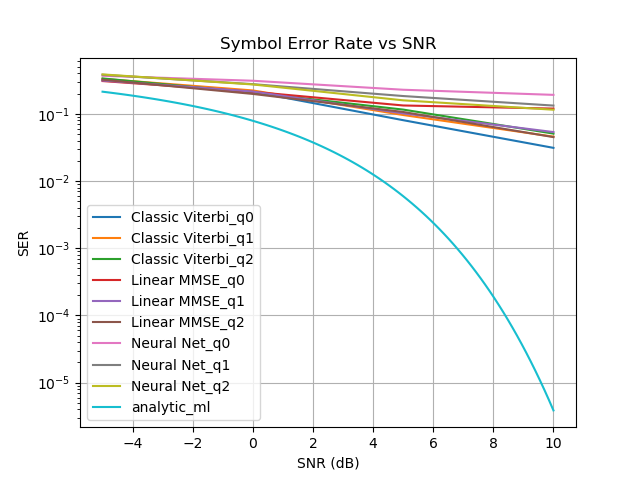
\includegraphics[width=\textwidth,height = 7cm]{results/quant_standard}


\item $p(y_{\mathrm{i}})$
: The randomness of the channel. As each received signal represents a state of the system to which noise may be added. A representative mixture-model can be estimated using a set of received signal training data. 
%picture of MM
%	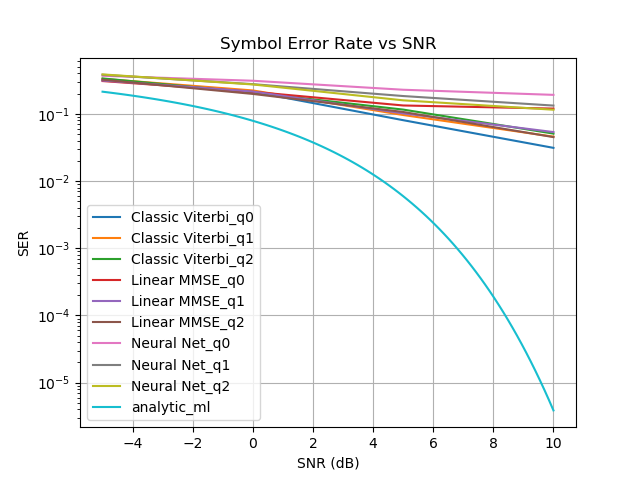
\includegraphics[width=\textwidth,height = 7cm]{results/quant_standard}


\item $p(\mathbf{x}_{\mathrm{i-L+1}}^{\mathrm{i}})$
: Assuming the transmitted symbols are equiprobable, this term can be neglected as all states $\mathbf{x}_{\mathrm{i-L+1}}^{\mathrm{i}}$ will have equal probability. 

\end{itemize}

In summary, the metrics required by the Viterbi algorithm permit use of a neural network and mixture model to estimate the conditional probability distribution function $p(y_{\mathrm{i}}|\mathbf{x}_{\mathrm{i-L+1}}^{\mathrm{i}})$
\subsection{A Reduced State ViterbiNet}
While the Viterbi Algorithm complexity complexity scales exponentially in the number of states possible at each step of the algorithm, in some cases this complexity can be reduced without significant degradation of performance. In particular, if the system is such that some states are redundant, these states can be combined. The following example with state redundancy is posed and one potential method of reducing these states is considered. 

A received signal 
\begin{equation}
y[k] = \sum_{\mathrm{l=1}}^{\mathrm{L}} a[l]x[k-l] + n[k], \; n[k]  \sim \mathcal{N}(0,1)
\end{equation}

with $x[k-l] \in \{ -1, +1\}$ and $n[k]  \sim \mathcal{N}(0,1)$.  

In the case of a causal, LTI system with inter-symbol-interference $\mathbf{a} = [.8,0,.02,.4]$ (normalized to have power 1) the received symbols is observed in figure \ref{fig:redundant_channel}. 

\begin{figure}[H]
	\includegraphics[width=10cm,height = 10cm]{system_model/redundant_channel}
	  \label{fig:redundant_channel}
	  	  \caption{LTI channel with state redundancy with high SNR}
\end{figure}

Originally, each step of the Viterbi algorithm would require searching through $2^L$ states. However, the low-power taps of the linear channel as well as the case of very even power taps of the channel result in redundancy. One way to exploit the redundancy is to cluster the original $2^L$ states into a set of $k$ clusters. The following algorithm is proposed for clustering.

    \noindent\rule[16pt]{\textwidth}{0.6pt}
	K-Means Clustering Algorithm:

    \noindent\rule[10pt]{\textwidth}{0.4pt}
    {\footnotesize
    \begin{tabbing}
        {\bf given} training data $y_{\mathrm{i}} \; \forall i \in {1..N}$, num Itr, and integer $K\leq N$. 
        \\*[\smallskipamount]
        {\bf for $i = 1..\# Itr$} \\
         \qquad \= {\bf for $y_{\mathrm{i}}\in {1..N}$\\
        \qquad \qquad \= 1.\ Label $y_{\mathrm{i}}$ as closest centroid k. 
        {\bf for centroid $k \in {1..K}$} \\
        \qquad \qquad \= 1.\ Move centroid $k$ to average of data points labeled $k$
        {\bf return} centroid locations
    \end{tabbing}}
    \noindent\rule[10pt]{\textwidth}{0.4pt}


- Need to note that the incoming signal is always kept at the front to preserve the survivor path step in the viterbi algorithm. 



\section{Simulation Results}
\subsection{System Model}

The following general system model was used in order to generate data used in testing the methods discuss above.


Consider the received signal 
\begin{equation}
y[k] = \sum_{\mathrm{l=1}}^{\mathrm{L}} a[l]x[k-l] + n[k], \; n[k]  \sim \mathcal{N}(0,1)
\end{equation}

with $x[k-l] \in \{ -1, +1\}$ and $n[k]  \sim \mathcal{N}(0,1)$.  
The resulting signal to noise ratio (SNR) is 
$\frac{E\{x[k]\}}{\sigma^2}$.


\begin{figure}[H]
	  \caption{Simulation Channels: LTI Channel}
	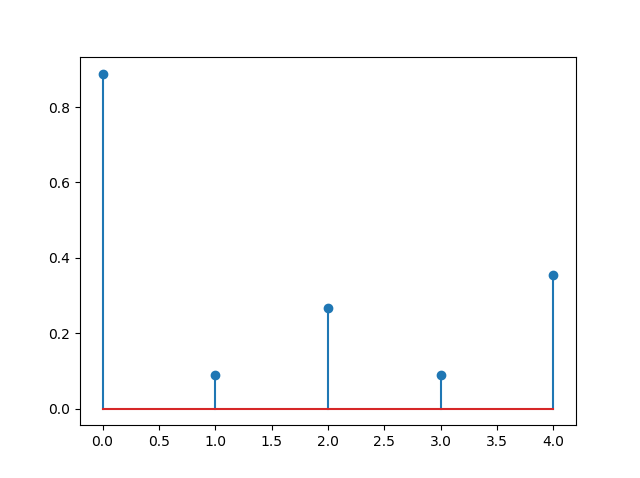
\includegraphics[width=10cm,height = 10cm]{system_model/lti_channel}
	  \label{fig:LTI Channel}
\end{figure}
\begin{figure}[H]
	  \caption{Simulation Channels: Quantizer}
	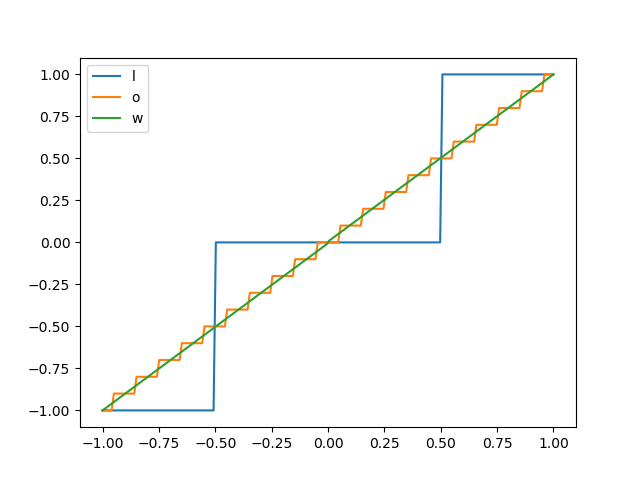
\includegraphics[width=10cm,height = 10cm]{system_model/quantizer}
	  \label{fig:Quantized Channel}
\end{figure}



Adding quantization at matched filter (prior to noise being added)


Details of NN architecture and training

Details of Mixture Model training

\subsection{Results}
proposed Figures
\begin{figure}[H]
	  \caption{LTI Channel performance}
	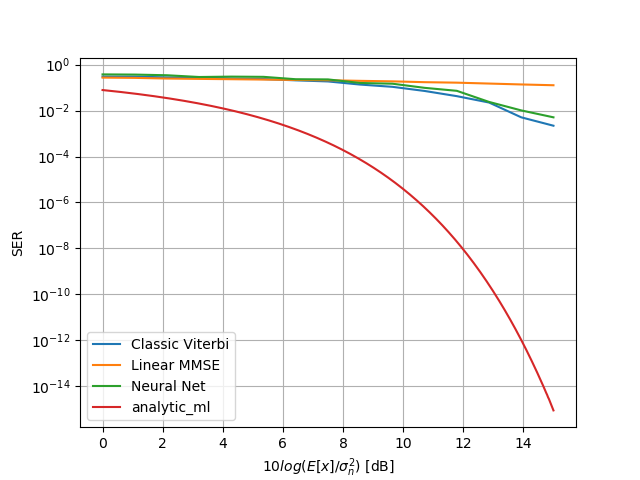
\includegraphics[width=\textwidth,height = 10cm]{results/lti_normal}
	  \label{fig:LTI Channel}
\end{figure}

\begin{figure}[H]
	  \caption{LTI + Quantized Channel performance}
	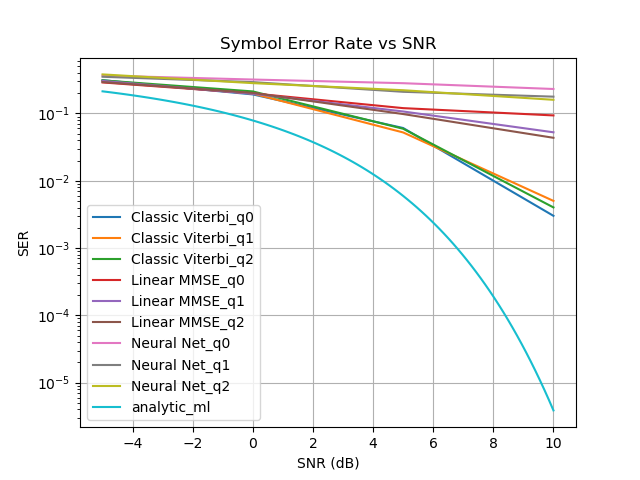
\includegraphics[width=\textwidth,height = 10cm]{results/lti_quantized}
	  \label{fig:LTI_quant Channel}
\end{figure}

\begin{figure}[H]
	  \caption{Reduced State ViterbiNet: LTI Channel}
	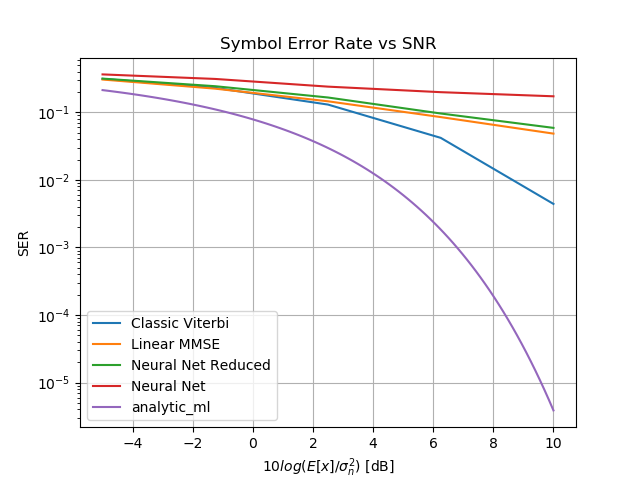
\includegraphics[width=\textwidth,height = 10cm]{results/lti_reduced}
	  \label{fig:reduced_lti}
\end{figure}

\begin{itemize}
\item ViterbiNet performance compared to MMSE and classic Viterbi LTI Channel

	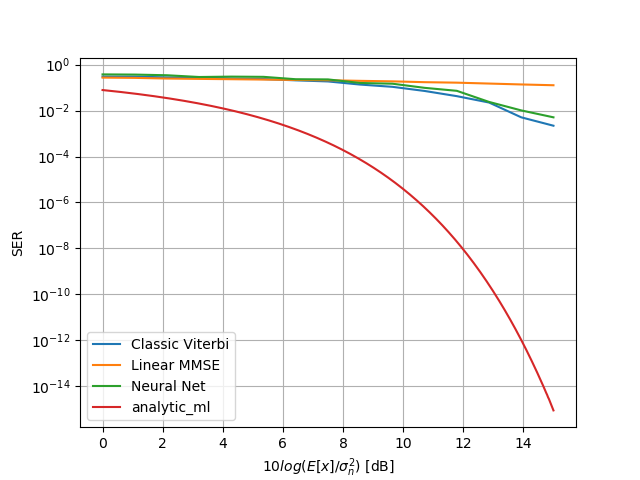
\includegraphics[width=\textwidth,height = 10cm]{results/lti_normal}

\item ViterbiNet performance compared to MMSE and classic Viterbi non-linear Channel

	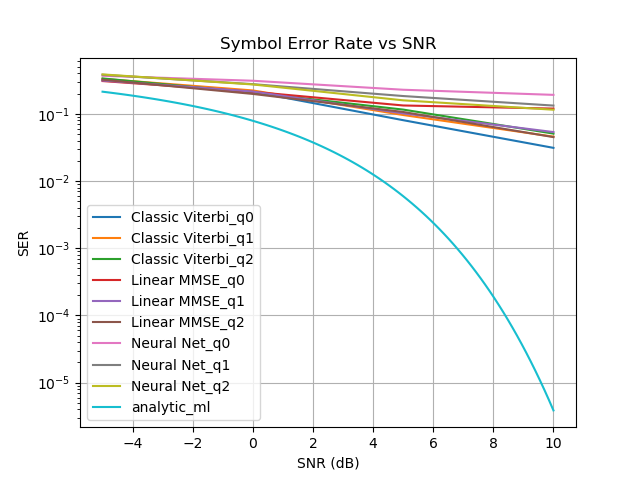
\includegraphics[width=\textwidth,height = 7cm]{results/quant_standard}

\item Reduced ViterbiNet on LTI Channel

	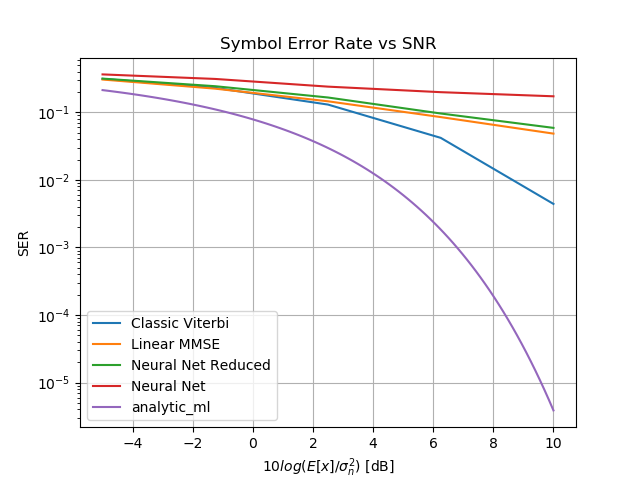
\includegraphics[width=\textwidth,height = 7cm]{results/lti_reduced}

\item Reduced ViterbiNet on non-linear Channel
%	\includegraphics[width=\textwidth,height = 7cm]{results/quant_reduced}

\end{itemize}
\subsection*{ViterbiNet}
\subsection*{Reduced State ViterbiNet}
\section{Conclusion}
\subsection{Future Work}
Discuss forward backward (App) algorithms that could be implemented.

\newpage
\bibliography{mc_report}
\end{document}